\begin{frame}{Aufgabe 5: Nichtfrequenzselektive Bedingungen}

\twocolumns{
  
  \begin{center}
    \includegraphics[width=\textwidth]{screenshots/Aufgabe5/1}
  \end{center}

}{

  \begin{center}
    \includegraphics[width=\textwidth]{screenshots/Aufgabe5/2}
  \end{center}

  
}{0.5\textwidth}
\end{frame}

\begin{frame}{Aufgabe 6: Frequenzselektive Bedingungen}
 \twocolumns{
  
  \begin{center}
    \includegraphics[width=\textwidth]{screenshots/Aufgabe6/1}
  \end{center}

}{

  \begin{center}
    \includegraphics[width=\textwidth]{screenshots/Aufgabe6/2}
  \end{center}

  
}{0.5\textwidth}

\end{frame}